\lecture{2009-12-01}

\subsubsection*{Übersicht}

\begin{itemize}
	\item $\ddot s + k^2s = 0$ ist Differentialgleichung (Dgl.) und "`verknüpft"' Funktionswerte und Ableitungen der unbekannten (gesuchten) Funktion $s(t)$
	\item Da nur eine unabhängige Variable (hier die Zeit $t$) existiert handelt es sich um eine gewöhnliche Differentialgleichung (\emph{ODE} -- ordinary differential equation).
	\item Da nur die Anfangswerte $s(0)$ und $\dot s(0)$ gegeben sind, ist es ein Anfangswerteproblem \emph{(AWP)} (engl. \emph{IVP} -- initial value problem).
	\begin{note}
		Existieren mehrere unabhängige Variablen ($x, y, z \in \mathbb{R}^3, t \in \mathbb{R}^+$), handelt es sich um eine partielle Differentialgleichung (\emph{PDE} -- partial differential equation).
	\end{note}
	\begin{example}
		\begin{itemize}
			\item Wärmeleitung: $u_t = \alpha^2 u_{xx}$\annotation{zur Notation: $u_{xx} \equals \frac{\partial^2}{\partial x^2}u(x,t)$, $u_t$ entsprechend}
			\item Wellengleichung: $u_{tt} = c^2 u_{xx}$
			\item Laplace-Gleichung: $\Delta u = u_{xx} + u_{yy} + u_{zz} = f(t, u)$
		\end{itemize}
	\end{example}
	\item $\ddot s + k^2s = 0$ ist eine DGL zweiter Ordnung, da die höchste enthaltene Ableitung zweiter Ordnung ist.
\end{itemize}

\subsubsection*{Fragen}
\begin{enumerate}
	\item Wie berechne ich \emph{eine} Lösung?
	\item Wie berechne ich \emph{alle} Lösungen?
	\item Definitionsbereich einer Lösung?
\end{enumerate}
Obige Fragen sind in der "`ODE-Welt"' beantwortbar, erfordern in der "`PDE-Welt"' hingegen 1-20 Jahre zur Lösung.

\paragraph{Spezielle Herangehensweise:} $\ddot s(t) + k^2s(t) = 0 \rightarrow$ Technik des intelligenten Ratens

\begin{example}[für $k = 1$]
\begin{align*}
	& \ddot s + s = 0 \\
	\leadsto &\text{ geraten: z. B. $s_1(t) = \sin(t)$, $s_2(t) = \cos(t)$}\\
	\implies &s_1(t) = \sin kt \\
	\implies &s_2(t) = \cos kt \\
	& \ddot s(t) + k^2s(t) = 0 \text { ist linear } \leadsto \text{ Überlagern ($Ax = 0$, $Ax = b$)} \\
	\implies &s(t) = c_1 \sin kt + c_2 \cos kt \text{ allgemeine Lösung, $c_1, c_2 \in \mathbb{R}$} \\
	\intertext{Parameter $c_1$, $c_2$ an Anfagswerte adaptieren}
	&\left. \begin{aligned}
		\leadsto s(0) &= 0 \implies c_2 = 0 \\
		\leadsto \dot s(0) &= v_0 \implies c_1k = v_0 \implies c_1 = \frac{v_0}{k}
	\end{aligned} \right\} \text {AWT $s(t) = \frac{v_0}{k}$ sinkt} \\
	&\left. \begin{aligned}
		s(t) &= c_1 \sin kt \\
		\dot s(t) &= c_1k \cos kt \\
		\ddot s(t) &= c_1k^2 \sin kt
	\end{aligned} \right\}\ddot s(t) + k^2s(t) = 0
\end{align*}
\end{example}

\subsubsection*{Schwingungsgleichung in $\mathbb{C}$: $\ddot s + k^2s = 0$}

\paragraph{Euler-Formel: $\euler^{\imag\varphi} = \cos \varphi + \imag \sin \varphi$}
\begin{align*}
	\frac{\diff}{\diff\varphi}\euler^{\imag\varphi} &= \frac{\diff}{\diff\varphi}(\cos \varphi + \imag \sin \varphi) = -\sin \varphi + \imag\cos \varphi \\
	\frac{\diff}{\diff\varphi}\euler^{\imag k\varphi} &= \frac{\diff}{\diff\varphi}(\cos k\varphi + \imag \sin k\varphi) =\\ &= -k\sin k\varphi + \imag k\cos k\varphi = \imag k(\cos k\varphi + \imag\sin k\varphi) = \imag k\euler^{\imag k\varphi} \\
	\frac{\diff^2}{\diff\varphi^2}\euler^{\imag k\varphi} &= \imag^2k^2\euler^{\imag k\varphi} = -k^2 \euler^{\imag k\varphi} \\
	S(t) &= C_1s_1(t) + C_2s_2(t) = C_1\euler^{\imag kt} + C_2\euler^{-\imag kt} \\&\text{ mit $C_1 = c_1 + \imag c_2$ und $C_2 = d_1 + \imag d_2$}
\end{align*}
Es gilt: $s(t) = \Re(S(t))$

\subsection{Anwendung der Differentiation}
Ziel: Kurvendiskussion von $f: I \rightarrow \mathbb{R}$ (differenzierbar)
\begin{definition}
	Lokales Maximum von $f$ in $x_0$ (im Inneren)
	\begin{equation*}
		f(x) \leq f(x_0) \quad |x - x_0| < \delta,\;\delta>0\text{ geg.}
	\end{equation*}
	Im Inneren: waagrechte Tangente $f(x_0) = 0$ charakterisiert lokales Extremum (notwendige Bedingung).
\end{definition}

\begin{center}
	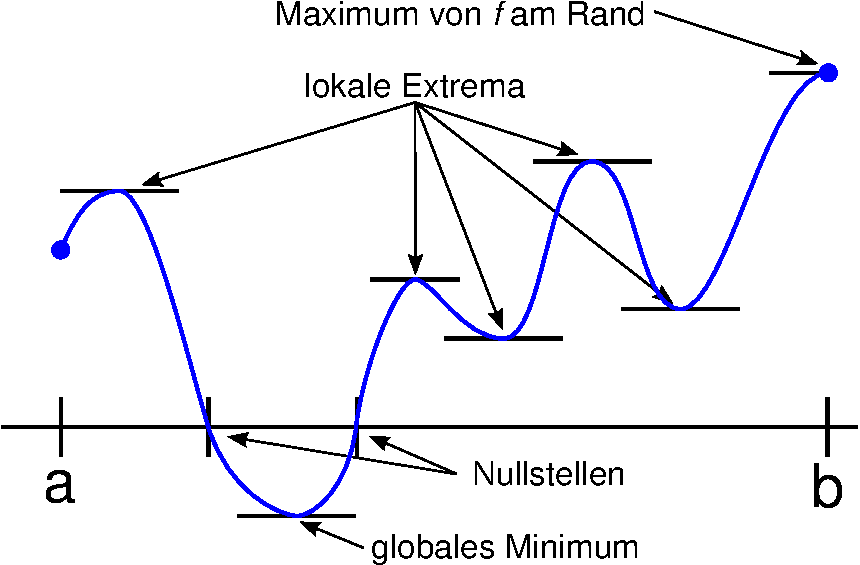
\includegraphics[width=0.6\textwidth]{include/20091201-1.pdf}
	\captionof{figure}{Nullstellen und Extrema}
\end{center}

\begin{note}
	$f(x) = x^3 \leadsto f'(0) = 0$, jedoch kein lokales Extremum
\end{note}

\subsubsection*{Satz von Rolle}
Voraussetzung: $f:[a, b] \rightarrow \mathbb{R}$ sei differenzierbar und es gilt $f(a) = f(b)$.
\begin{wrapfigure}[7]{r}[1cm]{0.4\textwidth}
 	\centering
	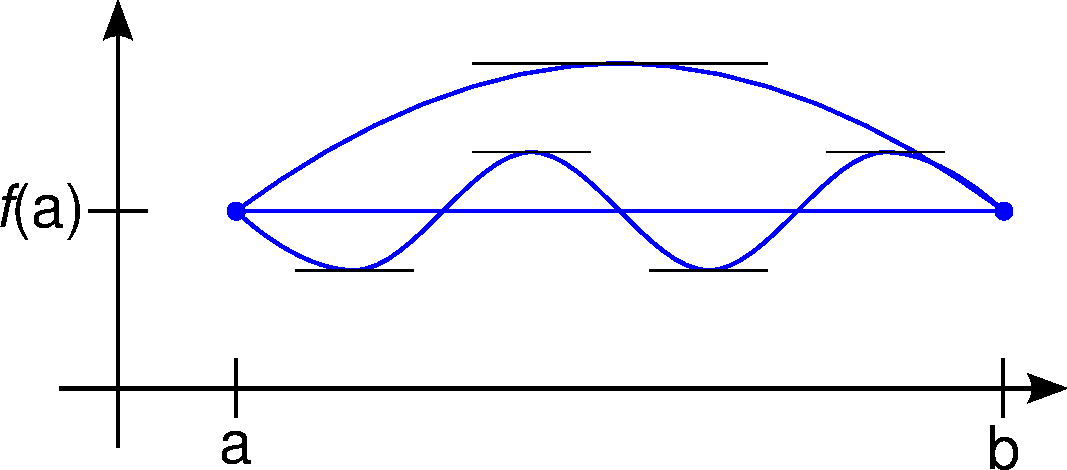
\includegraphics[width=0.4\textwidth]{include/20091201-2.pdf}
\end{wrapfigure}

\begin{theorem}
Es existiert ein $x_0$ mit $a < x_0 < b : f'(x_0) =~0$ oder $f$ ist konstant. Umgangssprachlich: "`$f$ ist entweder konstant oder besitzt ein Extremum."'
\end{theorem}

\noindent Uminterpretation: Sekantensteigung an Intervallenden: Es existiert ein $x_0$ mit gleicher Tangentensteigung.

\subsubsection*{1. Mittelwertsatz der Integralrechnung (1. MWS)}
Voraussetzung $f(a) = f(b)$ entfällt, aber es gilt: $f:[a,b] \rightarrow \mathbb{R}$ sei differenzierbar.

\begin{theorem}
Es existiert ein $x_0$ mit $a < x_0 < b$ so, dass die Sekantensteigung an den Endpunkten parallel zur Tangentensteigung in $x_0$ ist.
\begin{equation*}
	f'(x_0) = \frac{f(b) - f(a)}{b - a}
\end{equation*}
\end{theorem}
\begin{center}
	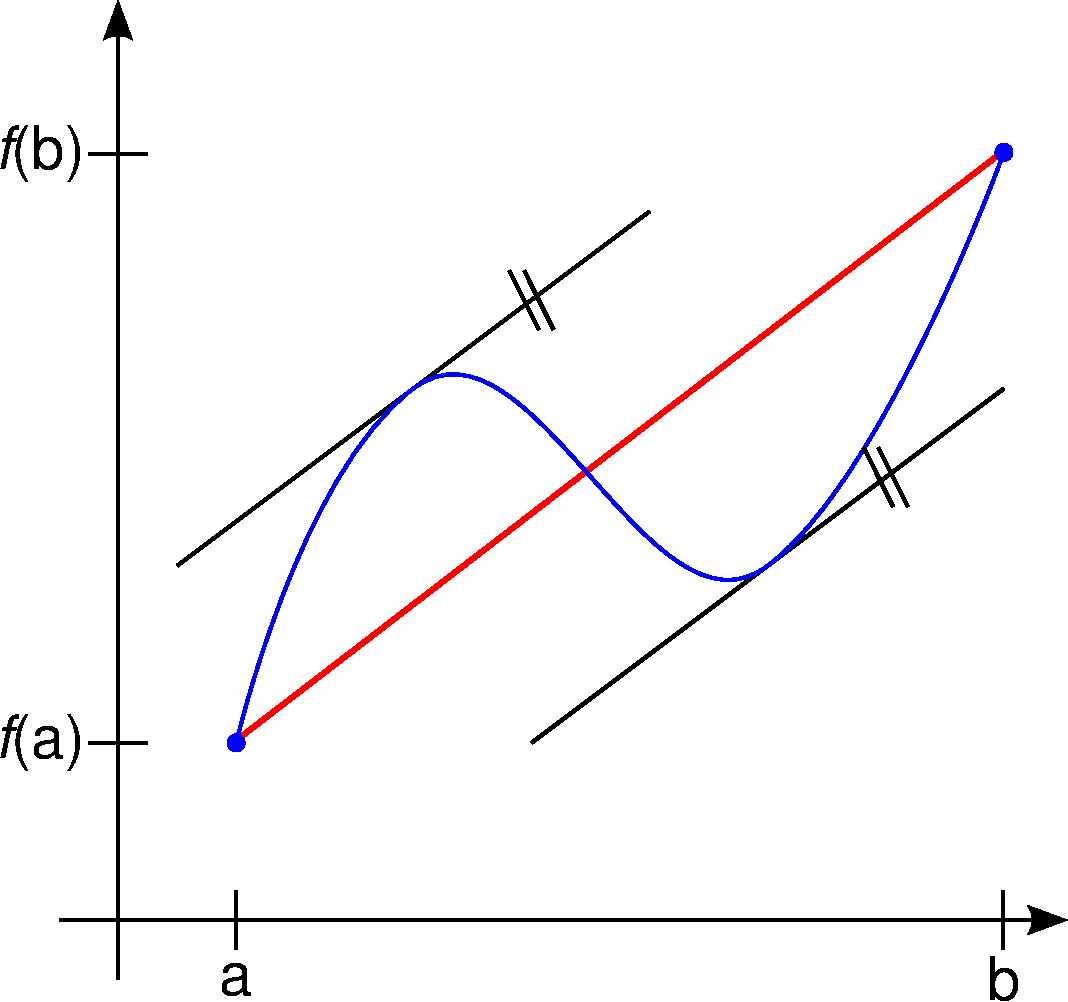
\includegraphics[width=0.4\textwidth]{include/20091201-3.pdf}
\end{center}
\begin{proof}
	Wende Satz von Rolle an auf:
	\begin{align*}
		h(x) &= f(x) - (x - a)\frac{f(b) - f(a)}{b - a} \\
		h'(x) &= f'(x) - 1\frac{f(b) - f(a)}{b - a} \\
		\intertext{Wie leicht zu sehen ist gilt:}
		h(a) &= f(a)\text{ und }h(b) = f(a) \\
		\intertext{aus dem Satz von Rolle folgt:}
		&\exists x_0 : h'(x_0) = 0 \implies f'(x_0) = \frac{f(b) - f(a)}{b - a}
	\end{align*}
\end{proof}
Folgerung für Differentialgleichungen:
\begin{equation*}
	\forall x : a < x < b \wedge f'(x) = 0 \implies f(x) = const \text{ einzige Lösung}
\end{equation*}
\begin{proof}[Beweis für 1. MWS]
	\begin{equation*}
		\exists x_0 : 0 = f'(x_0) = \frac{f(x) - f(a)}{x - a} \implies f(x) = f(a) = const
	\end{equation*}
	$\implies$ Konstante löst allgemein: $\dot s = 0 \implies s = c$.
\end{proof}

\subsubsection*{Monotone Funktionen}
\begin{enumerate}
	\item $f'(x) \geq 0 \implies f$ ist monoton wachsend
	\item $f'(x) \leq 0 \implies f$ ist monoton fallend
\end{enumerate}
\begin{example}
	z. z. \[f'(x_0) < 0 \implies x_1 > x_2 \implies f(x_1) < f(x_2)\]
	\[\cfrac{f(x_1) - f(x_2)}{\underbrace{x_1 - x_2}_{> 0}} = f'(x_0) < 0\]
\end{example}

\subsubsection*{Wendepunkte}
\begin{note}
	Die zweite Ableitung von $f$ beschreibt die Krümmung.
\end{note}
\begin{enumerate}
	\item $f''(x) > 0 \implies y = f(x)$ ist konvex (Linkskrümmung)
	\item $f''(x) < 0 \implies y = f(x)$ ist konkav (Rechtsskrümmung)
\end{enumerate}
Für den Wendepunkt gilt: $f''(x_0) = 0$ ist notwendig ($f'''(x_0) \neq 0$ ist hinreichend).
\begin{example}
	\begin{equation*}
		f(x) = x^3 \qquad f(0) = f'(0) = f''(0) = 0 \quad f'''(0) \equiv 6
	\end{equation*}
\end{example}
